\documentclass[catalan, a4paper]{scrartcl}

% encoding
\usepackage[utf8]{inputenc}
\usepackage[T1]{fontenc}
\usepackage{lmodern}
\usepackage{babel}

% formatting and fixes
\frenchspacing
\usepackage[style=spanish]{csquotes}
\MakeAutoQuote{«}{»}
\usepackage{subcaption}

% general design preferences (page, paragraph indent/space, margins, class options, ...)
\setlength{\parskip}{10pt}
\setlength{\parindent}{0pt}
%\pagestyle{plain}

% ADD ANY SPECIFIC PACKAGES HERE
% (CHEMISTRY, CODE, PUBLISHING)
\usepackage{siunitx}
\usepackage{tikz}
\usepackage{commath}
\usepackage{mathtools}
\usepackage{nicefrac}
\usepackage{minted}

% other options

%\usemintedstyle{xcode}
\setminted{
  %frame=leftline,
  %framesep=12pt,
  xleftmargin=15pt,
  breaklines,
  breakautoindent,
  breakindent=1em,
}

% hyperlink setup / metadata
\usepackage{hyperref}
\AfterPreamble{\hypersetup{
  pdftitle={Memòria P2 — PSAVC QP2019},
  pdfsubject={DAT},
}}

% document metadata
\author{Alba Mendez}
\title{Memòria pràctica 2\\
{\small DAT QT2019}}
\date{14 d'octubre de 2019}

\begin{document}

%\begin{minipage}{\columnwidth}
\maketitle
%\end{minipage}


\part{Introducció}

En aquesta pràctica es preten fer una breu introducció a Haskell, i
a la programació funcional pura en general.

Es comença explicant què
significa la programació funcional, què significa que sigui \emph{pura}
i què significa que sigui \emph{avaluada per necessitat}, com en el cas
de Haskell.

Llavors es presenta l'entorn de programació que es farà servir. Es
disposa d'un mòdul \mintinline{haskell}|Drawing| que ofereix una API
senzilla per pintar formes a través de fitxers SVG. També es disposa d'un
script \mintinline{text}|executaMain| que compila i executa el fitxer
de codi Haskell que li passem, generant els continguts del fitxer SVG
en la seva sortida estàndard.

\clearpage

\part{Haskell bàsic}

En aquest apartat s'explica com definir funcions, com funcionen les
definicions i alguns operadors.

\paragraph{Exercici 1.} Com a primer exercici es demana compilar un
programa senzill amb el mòdul \mintinline{haskell}|Drawing|:

\begin{minted}{haskell}
import Drawing

myDrawing :: Drawing
myDrawing = blank

main :: IO ()
main = svgOf myDrawing  
\end{minted}

El compilem i executem fent \mintinline{bash}|executaMain ex1.hs > ex1.svg|.
Llavors comprovem que, efectivament, es produeix un dibuix en
blanc (fig.~\ref{fig:ex1}).

\begin{figure}
\centering

\includegraphics[width=0.5\columnwidth]{../p2/ex1.pdf}
\caption{\label{fig:ex1} Resultat del primer exercici.}
\end{figure}

\clearpage

A continuació s'introdueixen algunes de les funcions de les que disposem
en el mòdul \mintinline{haskell}|Drawing|, notablement
\mintinline{haskell}|solidCircle|, \mintinline{haskell}|rectangle|,
\mintinline{haskell}|colored|, \mintinline{haskell}|translated| i
l'operador de composició: \mintinline{haskell}|<>|

\paragraph{Exercici 2.}

Es demana realitzar un programa que generi un semàfor amb tres llums
de colors vermell, groc i verd. Hem de fer-ho mitjançant una funció
\mintinline{haskell}|trafficLight| que dibuixi un llum a partir de 
dos paràmetres, el color i la posició en l'eix Y.

La implementació d'aquesta funció no té gaire misteri:

\begin{minted}{haskell}
lightBulb (y, c) = colored c $ translated 0 y $ solidCircle 1
\end{minted}

Abans de continuar, he vist necessari disposar d'una funció per composar
una llista de formes. A aquesta funció li he anomenat
\mintinline{haskell}|stack|, i es pot implementar fàcilment fent un fold:

\begin{minted}{haskell}
stack :: Foldable f => f Drawing -> Drawing
stack = foldr (<>) blank
\end{minted}

També he pensat que aniria bé una funció per mapejar una llista amb
una funció i després, composar les formes resultants. L'anomenaré
\mintinline{haskell}|dmap|:

\begin{minted}{haskell}
dmap :: (x -> Drawing) -> [x] -> Drawing
dmap f l = stack $ f <$> l
\end{minted}

Amb aquestes dues utilitats, escriure la resta del programa és tan
fàcil com:

\begin{minted}{haskell}
lights = [ (-2.5, green), (0, yellow), (2.5, red) ]
frame = rectangle 2.5 7.5 <> (colored gray $ solidRectangle 2.5 7.5)
trafficLight = dmap lightBulb lights <> frame

myDrawing = trafficLight
\end{minted}

El resultat final es pot veure a la fig.~\ref{fig:ex2}, i el codi complert
es troba a la pàgina~\pageref{code-ex2}.

\begin{figure}
\centering

\includegraphics[width=0.5\columnwidth]{../p2/ex2.pdf}
\caption{\label{fig:ex2} Resultat del segon exercici.}
\end{figure}

\clearpage
\part{Més sobre funcions}

\section{Funcions recursives}

En aquest apartat s'explica la necessitat de la recursivitat per expressar
repeticions en un llenguatge funcional. S'explica com definir funcions
recursives mitjançant pattern matching.

\paragraph{Exercici 3.} Es demana dibuixar un array de $3 \times 3$ semàfors.

%No cal fer servir funcions recursives per a això, ho podem fer simplement
%utilitzant \mintinline{haskell}|dmap|:

Només cal definir unes funcions utilitat, que repliquen objetes sobre un eix:

\begin{minted}{haskell}
row xs fig = dmap (\x -> translated x 0 fig) xs
col ys fig = dmap (\y -> translated 0 y fig) ys
\end{minted}

I combinar-les per obtenir l'array demanat:

\begin{minted}{haskell}
myDrawing = col [-8, 0, 8] $ row [-3, 0, 3] $ trafficLight
\end{minted}

El resultat final es pot veure a la fig.~\ref{fig:ex3}, i el codi complert
es troba a la pàgina~\pageref{code-ex3}.

\begin{figure}
\centering
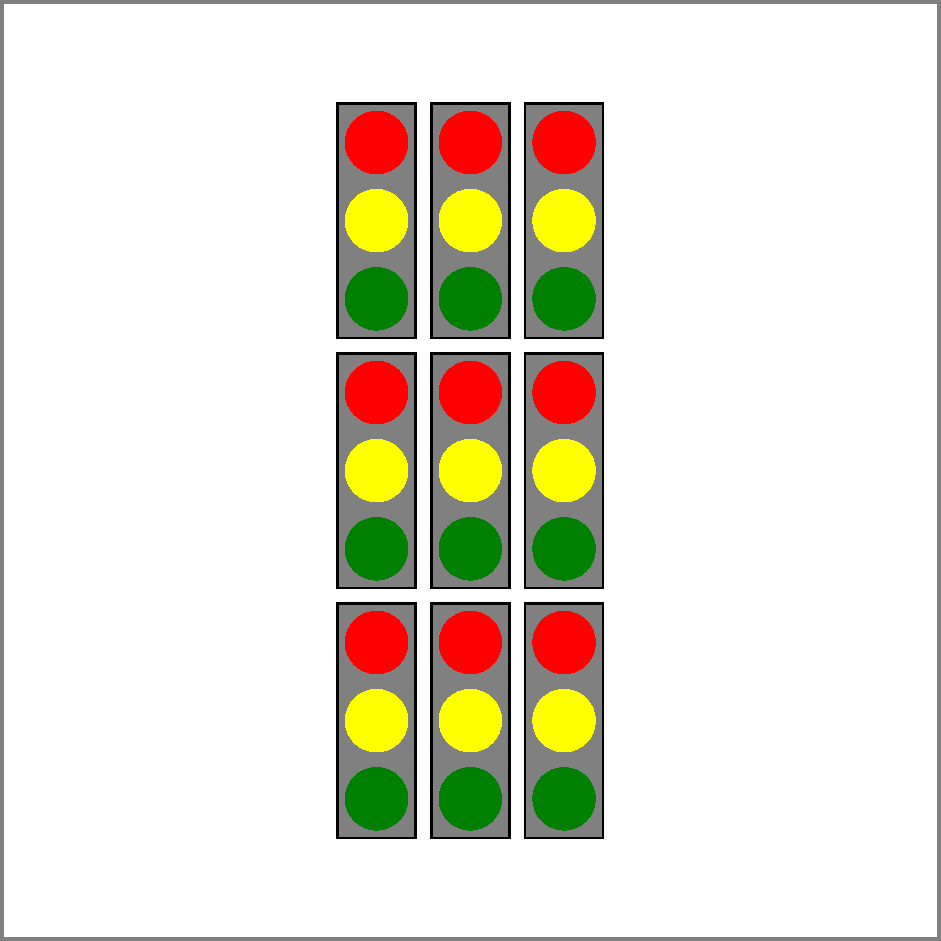
\includegraphics[width=0.5\columnwidth]{../p2/ex3.pdf}
\caption{\label{fig:ex3} Resultat del tercer exercici.}
\end{figure}

\paragraph{Exercici 4.}

Es demana ara dibuixar un arbre recursiu (veure resultat a la
fig.~\ref{fig:ex4a}).

Per fer-ho, definirem una funció recursiva que dibuixa:

\begin{itemize}
\item una línia cap a dalt de l'origen, de longitud 1
\item al final d'aquesta línia: dos subarbres,
  rotats \SI{18}{\degree} cap a cada sentit.
\end{itemize}

La funció queda així:

\begin{minted}{haskell}
tree 0 = blank
tree n = let
    subtree = dmap (\s -> rotated (s*pi/2/5) $ tree (n-1)) [1, -1]
  in polyline [(0,0), (0,1)] <> translated 0 1 subtree

myDrawing = tree 8
\end{minted}

El resultat es pot veure a la figura~\ref{fig:ex4a}.

Cal observar que aquesta definició \textbf{no} pinta una imatge
simètrica, ja que una de les dues branques es pinta per sobre
de l'altra. S'enten que això no és un problema, ja que la imatge
que es donava com a enunciat era també així.

Es demana ara que l'arbre tingui 'flors' grogues al final de les
branques. Això es pot aconseguir simplement canviant el cas zero
de la funció recursiva:

\begin{minted}{haskell}
tree 0 = colored yellow $ solidCircle 0.2
\end{minted}

El resultat final es pot veure a la fig.~\ref{fig:ex4b}, i el codi complert
es troba a la pàgina~\pageref{code-ex4}.

\begin{figure}
  \centering
  \begin{subfigure}{0.7\columnwidth}
  \centering
  
\includegraphics[width=.95\columnwidth]{../p2/ex4a.pdf}
  \caption{\label{fig:ex4a} Arbre recursiu de vuit nivells.}
  \end{subfigure}
  \begin{subfigure}{0.7\columnwidth}
  \centering
  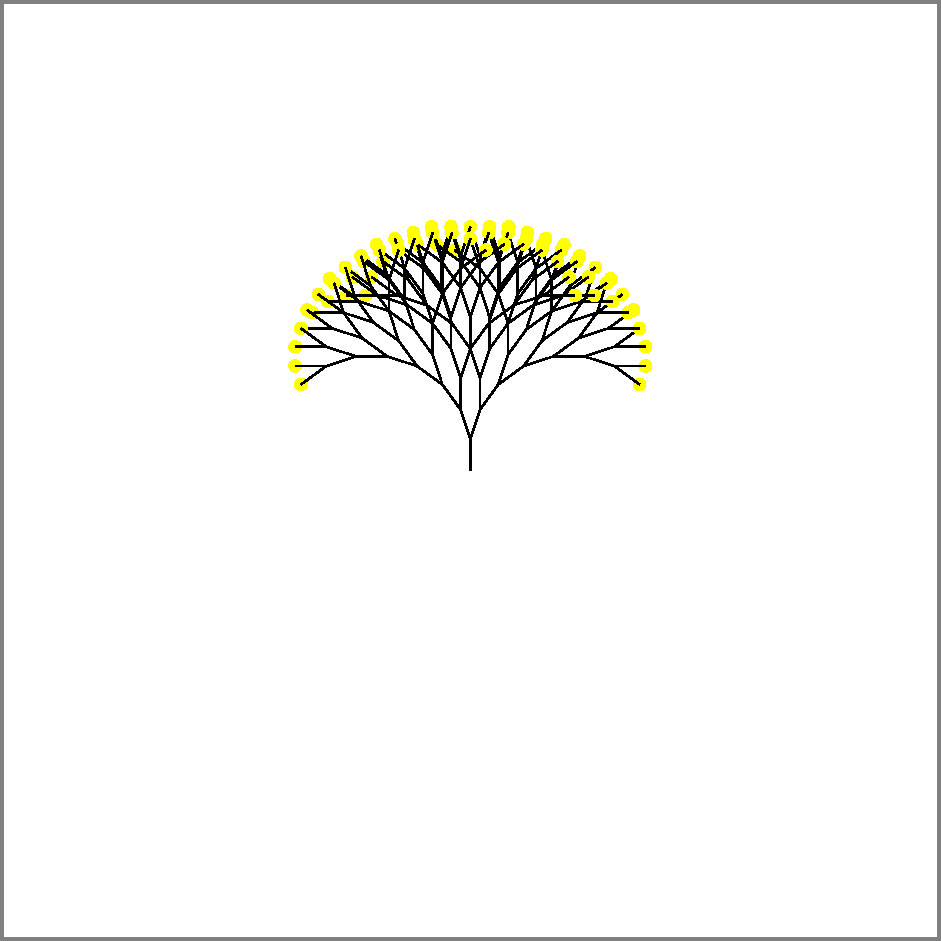
\includegraphics[width=.95\columnwidth]{../p2/ex4.pdf}
  \caption{\label{fig:ex4b} Arbre recursiu de vuit nivells, amb flors.}
  \end{subfigure}
  \caption{\label{fig:ex4} Resultat del quart exercici.}
\end{figure}

\section{Funcions d'ordre superior}

Ara s'introdueix el concepte de funció d'ordre superior (HOF) i la necessitat
que solucionen. Més endavant s'introdueixen algunes funcions d'ordre
superior incorporades a la llibreria estàndard de Haskell, i la classe
\emph{monoide}.

\paragraph{Exercici 5.}

Cal definir una funció \mintinline{haskell}|repeatDraw| que repetirà
la funció \mintinline{haskell}|thing| $n$ vegades, passant-li un enter
de $1$ a $n$ en cada repetició.

La funció és només una versió especial de \mintinline{haskell}|dmap|:

\begin{minted}{haskell}
repeatDraw :: (Int -> Drawing) -> Int -> Drawing
repeatDraw thing n = dmap thing [1..n]
\end{minted}

Ara l'exercici 3 es pot implementar així:

\begin{minted}{haskell}
myDrawing = repeatDraw lightRow 3

lightRow :: Int -> Drawing
lightRow r = repeatDraw (light r) 3

light :: Int -> Int -> Drawing
light r c = translated (3 * fromIntegral c - 6) (8 * fromIntegral r - 16) trafficLight
\end{minted}

Comprovem que es produeix el mateix resultat (fig.~\ref{fig:ex5}).
El codi complert es troba a la pàgina~\pageref{code-ex5}.

\begin{figure}
\centering
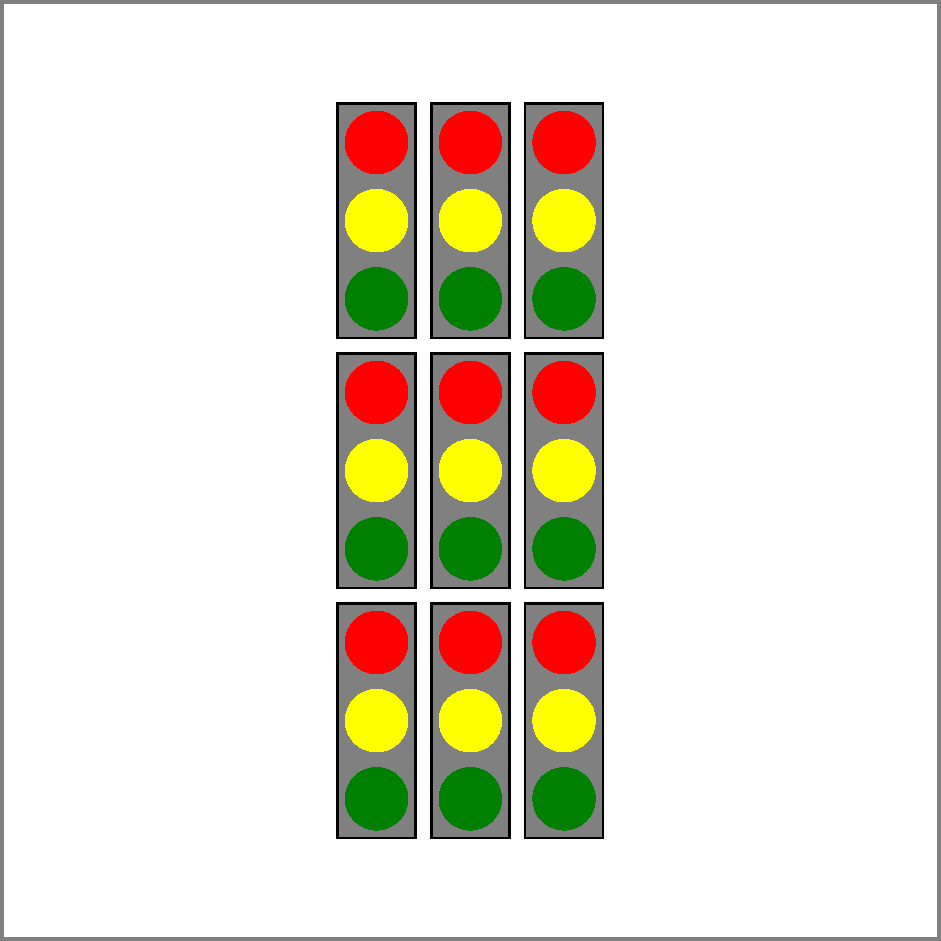
\includegraphics[width=0.5\columnwidth]{../p2/ex5.pdf}
\caption{\label{fig:ex5} Resultat del cinqué exercici.}
\end{figure}

\vskip 1.3em
Ara s'introdueix la classe \mintinline{haskell}|Monoid m|, s'explica
les operacions que implementa, i s'indica que \mintinline{haskell}|Drawable|
implementa aquesta classe.

Sabent que els dibuixos són monoides, m'adono que he reinventat la roda...
La meva funció \mintinline{haskell}|stack| fa el mateix que la funció
estàndard \mintinline{haskell}|mconcat|, i que \mintinline{haskell}|dmap|
fa el mateix que \mintinline{haskell}|foldMap|.

En altres paraules, l'exercici 2 també es pot escriure així:

\begin{minted}{haskell}
trafficLight = foldMap lightBulb lights <> frame
\end{minted}

\paragraph{Exercici 6.}

Es demana implementar una funció \mintinline{haskell}|trafficLights| que
accepti una llista de punts \mintinline{haskell}|[(Double, Double)]| i
dibuixi semàfors en cadascuna d'aquestes posicions, retornant el
\mintinline{haskell}|Drawable| resultant.

Només cal aplicar \mintinline{haskell}|foldMap| parcialment:

\begin{minted}{haskell}
trafficLights :: [(Double, Double)] -> Drawing
trafficLights = foldMap (\(x,y) -> translated x y trafficLight)
\end{minted}

Amb això també podem reescriure l'exercici 3, només ens cal generar
la llista de punts. Ho podem fer així:

\begin{minted}{haskell}
points = concat (for [-8, 0, 8] \r -> (for [-3, 0, 3] \c -> (c, r)))
\end{minted}

On la funció \mintinline{haskell}|for| és
\mintinline{text}|flip fmap|. Llavors només cal pintar
\mintinline{text}|trafficLights points|.
El resultat final es pot veure a la fig.~\ref{fig:ex6}, i el codi complert
es troba a la pàgina~\pageref{code-ex6}.

\begin{figure}
\centering
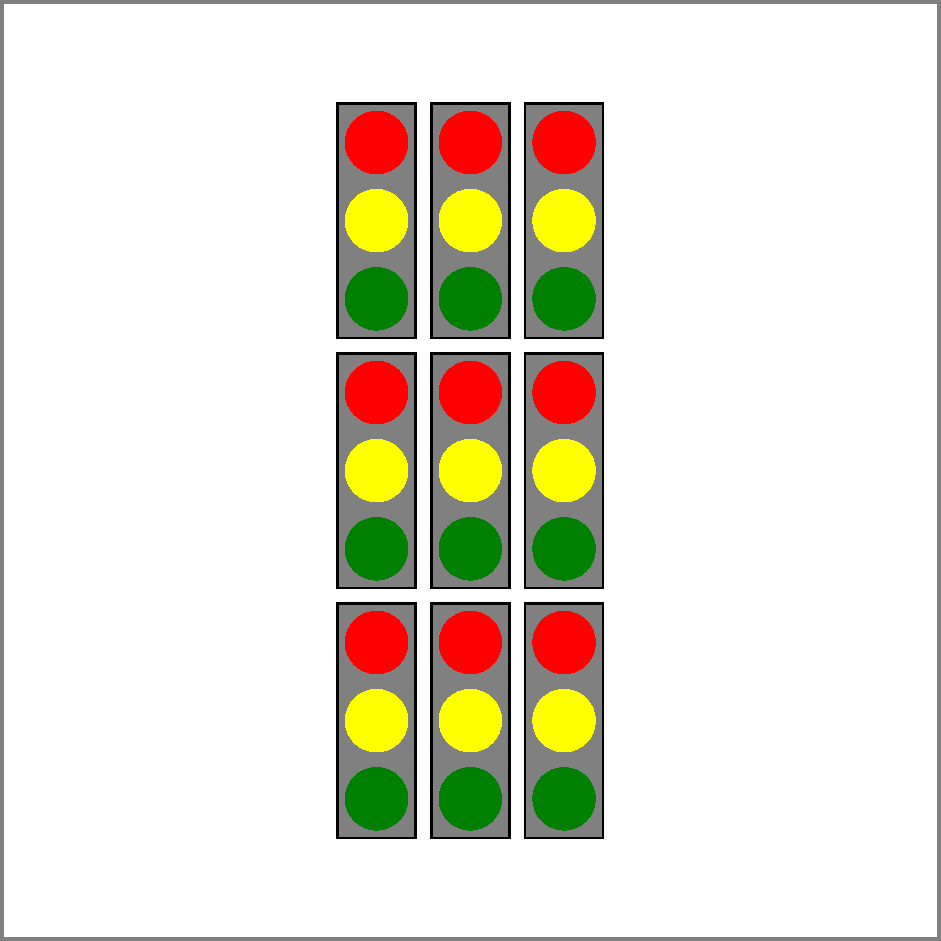
\includegraphics[width=0.5\columnwidth]{../p2/ex6.pdf}
\caption{\label{fig:ex6} Resultat del sisé exercici.}
\end{figure}


\clearpage
\appendix

\part{Codi complert}

\section*{\label{code-ex2} Exercici 2}

\inputminted{haskell}{../p2/ex2.hs}

\clearpage
\section*{\label{code-ex3} Exercici 3}

\inputminted{haskell}{../p2/ex3.hs}

\clearpage
\section*{\label{code-ex4} Exercici 4}

\inputminted{haskell}{../p2/ex4.hs}

\clearpage
\section*{\label{code-ex5} Exercici 5}

\inputminted{haskell}{../p2/ex5.hs}

\clearpage
\section*{\label{code-ex6} Exercici 6}

\inputminted{haskell}{../p2/ex6.hs}

\end{document}
